

%====================================================================
\section{Introduction}
\label{sec:intro}



%\newpage
%==================================================================


\section{Problem Definition}\label{sec:prob}
In Section~\ref{sec:intro}, we have talked about different biology applications that can be abstracted as a separability problem. In this section, we will formally formulate the problem and discuss the challenges in it. 

We first introduce some essential notations. Let $\mm$ be a feature-sample matrix of size $m\times N$, where each row is a feature and each column is a sample. Correspondingly, denote the $m$ features as $\ff=\{f_1,f_2,\cdots,f_m\}$ and $N$ samples as $\sss=\{s_1,s_2,\cdots,s_N\}$. Each entry $\mm_{i,j}$ in $\mm$ is of numeric type, referring to the value of sample $s_j$ on feature $f_i$. In addition, we are given two non-overlapping sets of samples, one with positive label and the other with negative label, denoted as $\sss_+$ and $\sss_-$ respectively. Both positive and negative samples are a subset of all samples, i.e., $\sss_+\subset \sss$ and $\sss_-\subset \sss$. Let $\bar{\sss}$ be the sample set with both positive and negative labels and $n$ be the total number of samples, i.e., $\sss_+\cup \sss_- = \bar{\sss}$, $|\bar{\sss}| = n$ and $n\leq N$. Furthermore, let $l_k$ be the label of sample $s_k\in \bar{\sss}$, i.e., $l_k=1$ if $s_k$ is positive and $l_k=-1$ if $s_k$ is negative. 

As illustrated in Figure~\ref{fig:workflow}, given matrix $\mm$ and two sample sets $\sss_+$ and $\sss_-$, the goal is to find discriminative features to separate $\sss_+$ from $\sss_-$, and output a visualization to explain the separability. In \genviz, we focus on finding \topk feature pairs instead of \topk single features. This is because \begin{inparaenum}[\itshape (a)\upshape]
\item a single feature can be considered as a special case of a feature pair by taking the same feature in a feature pair;
\item a combined feature pair is likely to provide new insight compared to single features;
\item feature pair can be easily visualized as a 2-D space.
\end{inparaenum}
As we will illustrate in Section~\ref{sec:exp}, two features that perform poorly on their own may have very good separability when combined together. Furthermore, since we are targeting as a data exploration tool before more time-consuming machine learning methods, our design principle is to prioritize running time over accuracy. Next, let us formally define the \textit{separability} problem. 

% \begin{figure}[h]
% 	\centering
% 	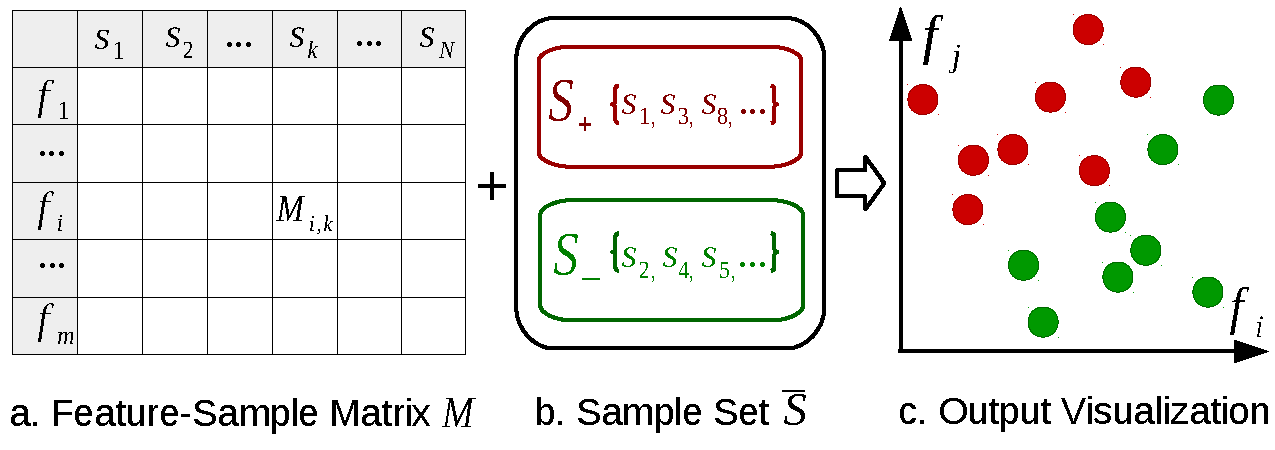
\includegraphics[width=\linewidth]{fig/workflow.pdf}
% \caption{\genviz Workflow}
% \label{fig:workflow}
% \end{figure} 

\begin{figure*}[t]
	\centering
	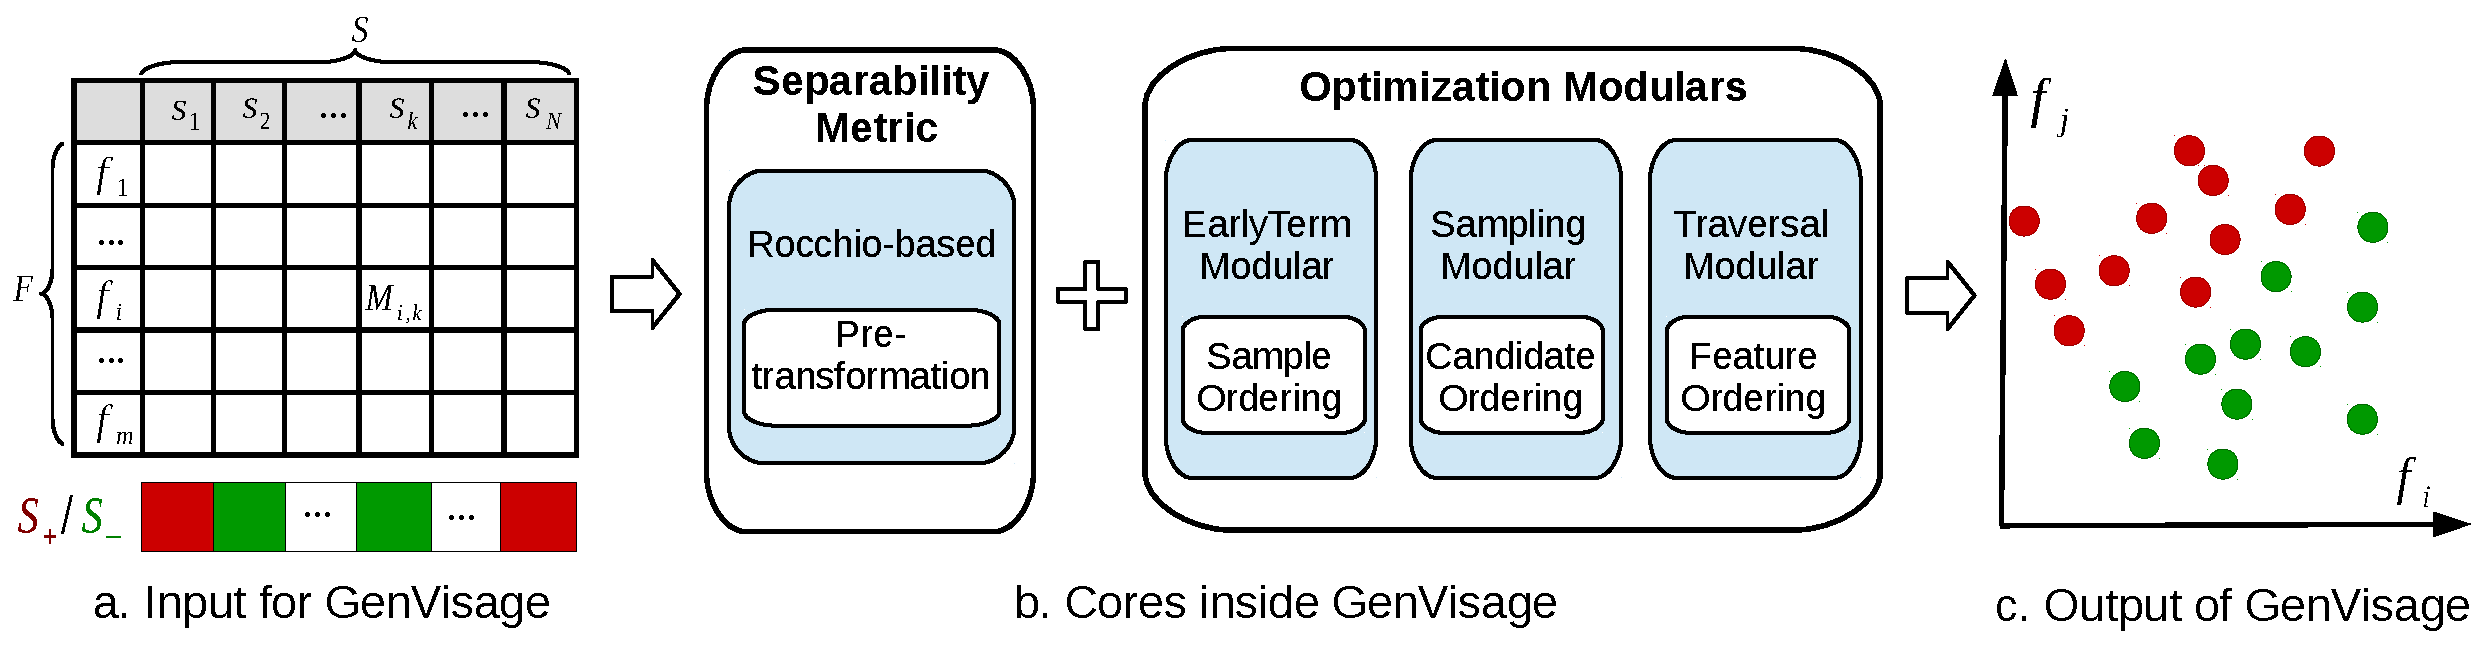
\includegraphics[width=0.9\linewidth]{fig/workflow2.pdf}
\caption{\genviz Workflow}
\label{fig:workflow}
\end{figure*} 



% \slhuang{feature pair is }
\begin{formulation}[Separability]\label{prob:separability}
Given a feature-sample matrix $\mm$ and two labeled sample set $(\sss_+,\sss_-)$, \textbf{fast identify} \topk feature pairs $(f_i,f_j)$ separating $\sss_+$ from $\sss_-$ based on a given \textbf{separability metric}, and output a 2-D \textbf{visualization}.
\end{formulation}
There are three key aspects in Problem~\ref{prob:separability}. First, the output of \genviz is not just the \topk feature pairs, but also the corresponding visualizations. The output visualizations can help the users better interpret the result, i.e., how $\sss_+$ is separated from $\sss_-$. Second, given a feature pair $(f_i,f_j)$, how to measure its quality in separating $\sss_+$ from $\sss_-$ poses an interesting challenge. Last but not least, how to fast identify \topk feature pairs based on the separability metric is also a big concern since small latency is critical for data exploration tool. In the following, we ellaborate more on these three points.

\stitle{Visualization Output.} Given a feature pair $(f_i,f_j)$, it is natural to visualize the sample sets $(\sss_+,\sss_-)$ in a two dimensional space by coloring $\sss_+$ as red and $\sss_-$ as green, where the x-axis and y-axis represent feature $f_i$ and $f_j$ respectively. Thus, a visualization and a feature pair has an one-to-one relationship: each visualization corresponds to one feature pair and vice versa. By looking at the visualization, the users can easily have a general sense of how $\sss_+$ and $\sss_-$ are separated for a given feature pair, and have a better interpretation towards the results compared to the pure feature pair names.


\stitle{Separability Metric.} As far as we are concerned, existing separability measurements focus on single feature instead of feature pair. For instance, in order to characterize differentially expressed genes (DEG), biologists typically do association test (e.g, hypergeometric test) to find the best single feature that separate two gene sets. However, we argue that feature pair can provide new insights that is not revealed by top single features, as we will demonstrate in Section~\ref{sec:exp}. Hence, developing a meaningful separability metric for feature pairs is the very first step towards our separability problem and is of great importance. Furthermore, since \genviz has visualization as the output instead of a pure separability score, our proposed separability metric should also encodes the visual separability to some extent. 

\stitle{Fast Identification.} Since \genviz serves as a data exploration tool before looking into more sophisticated machine learning algorithms, we in particular care more about the running time than the accuracy. For one thing, instead of complicated machine learning methods, we prefer light-weight separability metrics. In some sense, we try to solve Problem~\ref{prob:separability} in a "quick and dirty" way. For another, various optimization mechanisms are essential to further cut down the running time.

In the following, we will first describe our selected separability metric in Section~\ref{sec:metric}, and then discuss different optimization techniques in Section~\ref{sec:opt}.

%==================================================================
\section{Separability Metric}\label{sec:metric}
As discussed in Section~\ref{sec:prob}, given a feature pair $(f_i,f_j)$ we can visualize $\sss_+$ and $\sss_-$ in a 2-D space. In the following, we propose a separability metric based on linear separability~\cite{shamos1975geometric} for a 2-D visualization. 

Let us first review the concept of {\em linear separability} introduced in Euclidean geometry~\cite{shamos1975geometric}. A pair of point sets in two dimensions, i.e., $\sss_+$ and $\sss_-$, are \emph{linearly separable} if there exits at least one straight line in the plane such that all points from $\sss_+$ are on one side of the line, while all points from $\sss_-$ are on the other side of the line. Mathmatically, we can represent a line $\ell$ using Equation~\ref{eqn:line}, where $x$ and $y$ represent a sample's value on feature $f_i$ and $f_j$ respectively, and $w_0$, $w_i$ and $w_j$ are coefficients. Given a feature pair $(f_i,f_j)$ and a line $\ell$, let $\eta_{i,j}^{\ell,k}$ be the estimated label of a sample $s_k$. The estimated label $\eta_{i,j}^{\ell,k}$ is calculated according to Equation~\ref{eqn:est_label}: if $s_k$ lies on the upper side of $\ell$, then $\eta_{i,j}^{\ell,k}=1$; otherwise, $\eta_{i,j}^{\ell,k}=-1$.   
If there exists a line $\ell$ such that for any samples $s_k\in \bar{\sss}$, the estimated label $\eta_{i,j}^{\ell,k}$ is consistent with the real label $l_k$ as shown in Equation~\ref{eqn:linear}, then we say $\sss_+$ and $\sss_-$ are linear separable. 
\begin{equation}\label{eqn:line}
\begin{split}
\ell: \hspace{4mm} w_i\cdot x + w_j\cdot y +w_0 =0 
\end{split}
\end{equation}
\begin{equation}\label{eqn:est_label}
\eta_{i,j}^{\ell,k}=\sign(w_i\cdot \mm_{i,k} + w_j\cdot \mm_{j,k} +w_0)
\end{equation}
\begin{equation}\label{eqn:linear}
\eta_{i,j}^{\ell,k} = \left\{
                \begin{array}{ll}
                  1 \textit{\hspace{2mm} if \hspace{2mm}} s_k\in \sss_+, \textit{ i.e., } l_k=1 \\
                  -1 \textit{\hspace{2mm} if \hspace{2mm}} s_k\in \sss_-, \textit{ i.e., } l_k=-1 
                \end{array}
              \right.
\end{equation}



Next, let us introduce our proposed separability metric. Our proposed separability metric is based on linear separability and is defined as {\em how well a 2-D visualization can be linearly separated}. This is because \genviz stresses on visual explainability and linear separability in a 2-D visualization can be easily recognized and interpreted by the users. We then formally define the separability metric.
First, given a feature pair $(f_i, f_j)$ and a line $\ell$ in the 2-D plane, a sample $s_k$ is said to be correctly separated if Equation~\ref{eqn:linear} holds, i.e., $\eta_{i,j}^{\ell,k}\cdot l_k = 1$. Correspondingly, let $\tau_{i,j}^{\ell,k}$ be the variable indicating whether sample $s_k$ is correctly separated, as depicted in Equation~\ref{eqn:s_sample}. Then, given a feature pair $(f_i, f_j)$ and a line $\ell$, the separability score is defined as the number of correctly separated samples, denoted as $\theta_{i, j}^\ell$ as shown in Equation~\ref{eqn:s_line}. Figure~\ref{fig:brute_force} shows some possible $\theta_{i, j}^\ell$ with different separating lines. Finally, the separability score for a feature pair $(f_i,f_j)$ is defined as the largest $\theta_{i, j}^{\ell}$ among all possible lines $\ell$, denoted as $\theta_{i, j}$ as shown in Equation~\ref{eqn:s_viz}. 
\begin{equation}\label{eqn:s_sample}
\tau_{i,j}^{\ell,k}=\left\{
                \begin{array}{ll}
                  1 \textit{\hspace{2mm} if \hspace{2mm}} \eta_{i,j}^{\ell,k}\cdot l_k = 1\\
                  0 \textit{\hspace{2mm} otherwise \hspace{2mm}} 
                \end{array}
              \right.
\end{equation}
\begin{equation}\label{eqn:s_line}
\theta_{i,j}^{\ell}= \sum_{k}{\tau_{i,j}^{\ell,k}}
\end{equation}
\begin{equation}\label{eqn:s_viz}
\theta_{i,j}= \max_{\ell}\{\theta_{i,j}^{\ell}\}
\end{equation}

%The basic intuition is that the users can easily recognize and interpret linear separability in a 2-D visualization. Thus if a visualization is perfectly linearly separated, it should have high score in our proposed separability metric; otherwise, we would find the best separating line $\ell$ in the visualization and report the largest number of correctly separated samples as the separability score.\silu{talk about weighted case}

\stitle{Brute Force.} As illustrated in Figure~\ref{fig:brute_force}, a brute force way to calculate $\theta_{i,j}$ is to first enumerate all possible separating lines $\ell$ and calculate each $\theta_{i,j}^\ell$. This is infeasible as there are infinite number of possible lines. However, we can easily trim down the search space to $O(n^2)$ lines by linking every two points in the 2-D plane. This is because the results of all other possible lines can be covered by these $O(n^2)$ lines. Nevertheless, it is still very time-consuming to consider $O(n^2)$ lines for each feature pair $(f_i,f_j)$. We further propose to use a {\em representative line} $\hat{\ell}$ to approximate $\theta_{i, j}$ as shown in Equation~\ref{eqn:s_viz_appr}, instead of considering all $O(n^2)$ possible lines and pick the best in Equation~\ref{eqn:s_viz}. Now, the search space is reduced to $O(1)$ from $O(n^2)$. The representative line is picked based on Rocchio's algorithm~\cite{rocchio1971relevance}. As we will show later in Section~\ref{sec:exp}, $\theta_{i,j}^{\hat{\ell}}$ is comparable to $\theta_{i,j}$ when using Rocchio-based representative line $\hat{\ell}$. Let us describe in detail about the Rocchio-based representative line.
\begin{equation}\label{eqn:s_viz_appr}
\theta_{i,j}  \approx \theta_{i,j}^{\hat{\ell}}
\end{equation}

\stitle{Rocchio-based.} The basic idea of Rocchio's algorithm is to estimate each sample's label the same as its nearest centroid. More specifically, let us denote the centroid of positive samples $\sss_+$ and negative samples $\sss_-$ as $\mu_+=(\mm_i^+,\mm_j^+)$ and $\mu_-=(\mm_i^-,\mm_j^-)$ respectively ,as shown in Figure~\ref{fig:rocchio}. Link $\mu_+$ with $\mu_-$, then the perpendicular bisector is defined as the representative separating line $\hat{\ell}$. Mathmatically, $\hat{\ell}$ can be represented as an instantiated line in Equation~\ref{eqn:line} with instantiated $w_i$, $w_j$ and $w_0$ as shown in Equation~\ref{eqn:rep_line}. Figure~\ref{fig:rocchio} illustrates the centroids $\mu_+$ and $\mu_-$, as well as the Rocchio-based representative separating line $\hat{\ell}$. The corresponding $\theta_{i,j}^{\hat{\ell}}$ equals 13 with one negative sample (blue point in Figure~\ref{fig:rocchio}) mis-estimated as positive.


%\hat{\ell}: \hspace{4mm} (\mm_i^+-\mm_i^-)\cdot x + (\mm_j^+-\mm_j^-)\cdot y -(\frac{(\mm_i^+)^2-(\mm_i^-)^2}{2}+\frac{(\mm_j^+)^2-(\mm_j^-)^2}{2}) =0 

\begin{equation}\label{eqn:rep_line}
\begin{split}
& w_i = \mm_i^+-\mm_i^- \\
& w_j = \mm_j^+-\mm_j^- \\
& w_0 = -(\frac{(\mm_i^+)^2-(\mm_i^-)^2}{2}+\frac{(\mm_j^+)^2-(\mm_j^-)^2}{2})
\end{split}
\end{equation}

\begin{figure}[h]
	\centering
	\begin{subfigure}{0.235\textwidth}
		\centering
		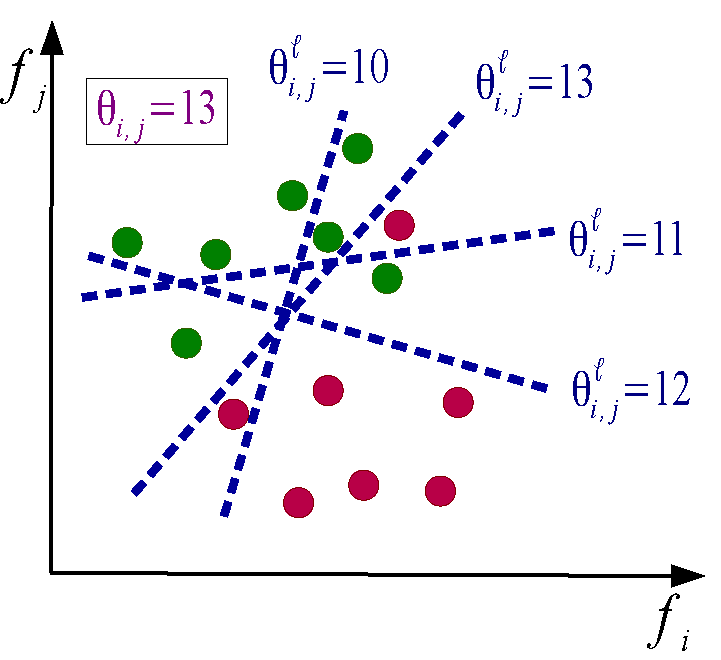
\includegraphics[width=\linewidth]{fig/metric.pdf}
		\vspace{-5mm}
		\caption{Brute Force}%{$\theta_{i,j}^{\ell}$ with Different Lines}
		\label{fig:brute_force}
	\end{subfigure}
	\begin{subfigure}{.235\textwidth}
		\centering
		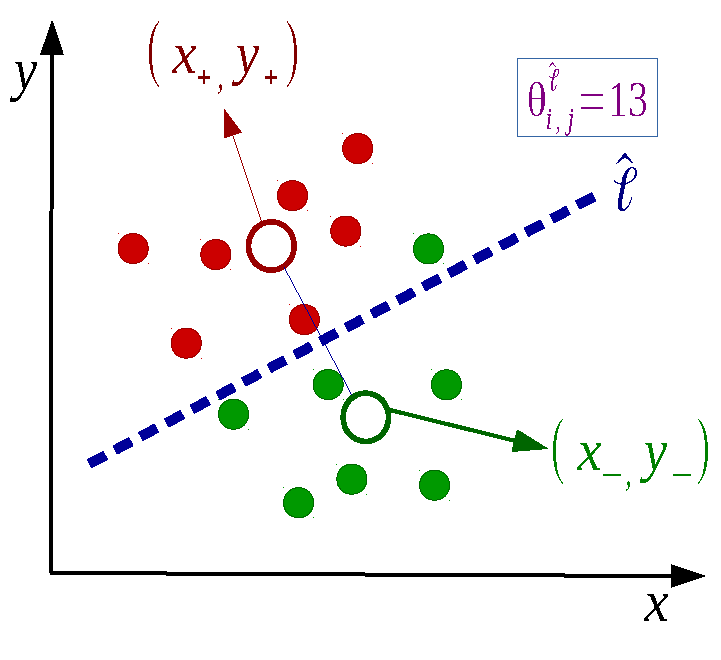
\includegraphics[width=\linewidth]{fig/rocchio.pdf}
		\vspace{-5mm}
		\caption{Rocchio-Based}%{$\theta_{i,j}^{\hat{\ell}}$ with Representative Line}
		\label{fig:rocchio}
	\end{subfigure}
\caption{Different methods to Calculate Separability Score $\theta_{i,j}$}
\label{fig:metric}
\end{figure} 

\stitle{Brute-force v.s. Rocchio-based.} Compared to brute force, Rocchio-based method is more light-weight in terms of running time, but at the cost of accuracy in calculating $\theta_{i,j}$. Intuitively, Rocchio-based representative line is a reasonable approxy to the best separating line since Rocchio-based method assigns each sample to its nearest centroid and each centroid is calculated as the representative of each group. We will further experimentally demonstrate that $\theta_{i,j}-\theta_{i,j}^{\hat{\ell}}$ is small in Section~\ref{sec:exp}.

%==================================================================
\section{Proposed Optimizations}\label{sec:opt}
In the following, we will focus on Rocchio-based method to calculate the separability score. We first analyze the time complexity and then propose several optimization techniques in order to reduce the running time. 

\stitle{Time Complexity Analysis.} Given a feature pair $(f_i, f_j)$, the separating line $\hat{\ell}$ can be calculated in $O(1)$ using Equation~\ref{eqn:rep_line}. However, calculating the number of correctly separated samples $\theta_{i,j}^{\hat{\ell}}$ requires a full scan of all samples, i.e., $O(n)$. In addition, by choosing any two features from the whole feature set, there are $O(m^2)$ feature pair candidates. Thus, in total the running time complexity is $O(m^2n)$, which is very time-consuming especially when $m$ and $n$ are large. In the following, we propose different methodologies to reduce the running time.

First, we observe massive redundancy in calculating Equation~\ref{eqn:rep_line} for different feature pairs. In Section~\ref{ssec:trans}, we propose to map sample-feature matrix $\mm$ into a different space, and then transform Equation~\ref{eqn:rep_line} accordingly. Next, we introduce several different optimization modulars to further reduce the running time in Section~\ref{ssec:earlyT},~\ref{ssec:sampling} and \ref{ssec:traversal}. Modular \earlyT and \sampling aim to reduce the number of samples checked (i.e., $n$), while modular \traversal aims to reduce the number of feature pairs checked (i.e., $m^2$). These optimization modulars can be used by their own or combined together, as we will show in Section~\ref{sec:exp}. 

\subsection{Pre-Transformation} \label{ssec:trans}
\stitle{Motivation.} Let us first review the process of computing the separability score $\theta_{i,j}^{\hat{\ell}}$. Given a fature pair $(f_i,f_j)$, we first compute $w_0$, $w_i$ and $w_j$ for $\hat{\ell}$ based on Equation~\ref{eqn:rep_line}. Next, for each sample $s_k$, we can get the estimated label $\eta_{i,j}^{\hat{\ell},k}$ according to Equation~\ref{eqn:est_label}. This step requires two multiplications and three additions. Last, we can calculate $\tau_{i,j}^{\hat{\ell},k}$ and the separability score $\theta_{i,j}^{\hat{\ell}}$ based on Equation~\ref{eqn:s_sample} and \ref{eqn:s_line} respectively. The whole process is repeated for every feature pair candidate. However, we observe that there exists massive redundancy when calculating different feature pairs. For instance, given two feature pairs $(f_i,f_j)$ and $(f_i,f_{j'})$ with fixed $f_i$, $w_i$ is in fact the same, and $w_i\cdot \mm_{i,k}$ in Equation~\ref{eqn:est_label} is repeated twice for each sample $s_k$. Thus, we propose to pre-transform $\mm_{i,k}$ into another space to reduce the computational redundancy.

\stitle{Transformation.} For each $\mm_{i,k}$, i.e., the value of sample $s_k$ on feature $f_i$, we pre-transform it to $\widehat{\mm}_{i,k}$ as illustrated in Equation~\ref{eqn:matrix_transform}, where $\mm_i^+$ ($\mm_j^+$) and $\mm_i^-$ ($\mm_j^-$) are constants given a feature $f_i$ ($f_j$). By incorporating $\ell_k$ in Equation~\ref{eqn:matrix_transform}, we can unify the process of calculating $\tau_{i,j}^{\hat{\ell},k}$ for both positive and negative samples, and get rid of checking the real label $\ell_k$ in Equation~\ref{eqn:s_sample}. Accordingly, Equation~\ref{eqn:est_label} and Equation~\ref{eqn:s_sample} can be combined and transformed into Equation~\ref{eqn:s_sample_transform}.

\begin{equation}\label{eqn:matrix_transform}
\widehat{\mm}_{i,k} = ((\mm_i^+-\mm_i^-)\cdot \mm_{i,k}-\frac{(\mm_i^+)^2-(\mm_i^-)^2}{2})\cdot \ell_k 
\end{equation}

\begin{equation}\label{eqn:s_sample_transform}
\tau_{i,j}^{\hat{\ell},k}=\left\{
                \begin{array}{ll}
                  1 \textit{\hspace{2mm} if \hspace{2mm}} \sign(\widehat{\mm}_{i,k} + \widehat{\mm}_{j,k}) = 1\\
                  0 \textit{\hspace{2mm} otherwise \hspace{2mm}} 
                \end{array}
              \right.
\end{equation}

%\begin{equation}\label{eqn:est_label_transform}
%\eta_{i,j}^{\hat{\ell},k}=\sign(\widehat{\mm}_{i,k} + \widehat{\mm}_{j,k})
%\end{equation}

Now, let us revisit the process of computing separability score $\theta_{i,j}^{\hat{\ell}}$ after pre-transformation. Given a feature pair $(f_i,f_j)$, we can compute $\tau_{i,j}^{\hat{\ell},k}$ for each sample $s_k$ based on Equation~\ref{eqn:s_sample_transform}. Note that this step only involves one addition and one comparison. Then, similar to that without transformation, we can calculate $\theta_{i,j}^{\hat{\ell}}$ based on Equation~\ref{eqn:s_line}. In all, compared to that without transformation, we not only eliminate the step of computing $w_0$, $w_i$ and $w_j$ for every feature pair, but also reduce the cost of calculating $\eta_{i,j}^{\hat{\ell},k}$ in Equation~\ref{eqn:est_label}. Hence, by conducting transformation in Equation~\ref{eqn:matrix_transform} and~\ref{eqn:s_sample_transform}, we have mapped our problem to a new space. In the following sections, we will consider $\widehat{\mm}$ instead of $\mm$, and Equation~\ref{eqn:s_sample_transform} instead of Equation~\ref{eqn:est_label} and~\ref{eqn:s_sample}.

\subsection{Early Termination} \label{ssec:earlyT}
As discussed at the beginning of Section~\ref{sec:opt}, given a feature pair $(f_i,f_j)$, we need to make a full scan of all samples to compute $\theta_{i,j}^{\hat{\ell}}$. However, since we only care about 

\stitle{High Level Idea.}

\stitle{Enhancement by Sample Ordering.}

\earlyT Modular
Early Termination

\subsection{Sampling-based Estimation} \label{ssec:sampling}
Sampling-based Estimation
\sampling Modular

\subsection{Search Space Traversal} \label{ssec:traversal}
\traversal Modular

%==================================================================
\section{Experiment}
\label{sec:exp}








